 \section{Python Dictionary}
\vspace{12pt}
\noindent 
Setiap kunci dipisahkan dari nilainya oleh titik dua (:), item dipisahkan oleh koma, dan semuanya tertutup dalam kurung kurawal. Kamus kosong tanpa barang ditulis hanya dengan dua kurung kurawal, seperti ini:  $  \{  $ $  \}  $. \par
\noindent 
Kunci unik dalam kamus sementara nilai mungkin tidak. Nilai kamus bisa berupa tipe apa pun, namun kunci harus berupa tipe data yang tidak berubah seperti string, angka, atau tupel. \par
\vspace{12pt}
\noindent 
\vspace{\baselineskip}
Accessing Values in Dictionary: \par
\noindent 
Untuk mengakses elemen kamus, Anda dapat menggunakan tanda kurung siku yang sudah dikenal bersama dengan kunci untuk mendapatkan nilainya. Berikut adalah contoh sederhana - \par
\noindent 
\begin{verbatim}

 \hspace*{0.5in}  $  \#  $!/usr/bin/python \par
\vspace{12pt}
\noindent 
 dict =  $  \{  $'Name': 'Zara', 'Age': 7, 'Class': 'First' $  \}  $ \par
\vspace{12pt}
\noindent 
 print "dict['Name']: ", dict['Name'] \par
\noindent 
 print "dict['Age']: ", dict['Age'] \par
\noindent 
Bila kode diatas dieksekusi, maka menghasilkan hasil sebagai berikut - \par
\noindent 
 dict['Name']:~ Zara \par
\noindent 
 dict['Age']:~ 7 \par
\noindent 
Jika kita mencoba mengakses item data dengan sebuah kunci, yang bukan bagian dari kamus, kita mendapatkan error sebagai berikut - \par
\noindent 
 $  \#  $!/usr/bin/python \par
\vspace{12pt}
\noindent 
 dict =  $  \{  $'Name': 'Zara', 'Age': 7, 'Class': 'First' $  \}  $ \par
\vspace{12pt}
\noindent 
 print "dict['Alice']: ", dict['Alice'] \par
\noindent 
Bila kode diatas dieksekusi, maka menghasilkan hasil sebagai berikut - \par
\noindent 
 dict['Alice']: \par
\noindent 
 Traceback (most recent call last): 
\noindent 
 File "test.py", line 4, in <module>  
 print "dict['Alice']: ",     dict['Alice'];  
 KeyError: 'Alice' 
\end{verbatim}
\vspace{12pt}
\noindent
\vspace{\baselineskip}
Updating Dictionary \par
\noindent 
Anda dapat memperbarui kamus dengan menambahkan entri baru atau pasangan nilai kunci, memodifikasi entri yang ada, atau menghapus entri yang ada seperti yang ditunjukkan di bawah ini dalam contoh sederhana - \par
\noindent 
\vspace{12pt}
\vspace{\baselineskip}
\vspace{\baselineskip}
\begin{verbatim}
 $  \#  $!/usr/bin/python \par
\vspace{12pt} 
  dict =  $  \{  $'Name': 'Zara', 'Age': 7, 'Class': 'First' $  \}  $ 
\vspace{12pt}

  dict['Age'] = 8;  $  \#  $ update existing entry 
  dict['School'] = "DPS School";  $  \#  $ Add new entry  
  print "dict['Age']: ", dict['Age'] 
 print "dict['School']: ", dict['School'] 
Bila kode diatas dieksekusi, maka menghasilkan hasil sebagai berikut - 
 dict['Age']:~ 8 \par 
 dict['School']:~ DPS School 
 \end{verbatim}
 
\vspace{12pt}
\noindent 
Delete Dictionary Elements \par
\noindent 
Anda dapat menghapus elemen kamus individual atau menghapus keseluruhan isi kamus. Anda juga dapat menghapus seluruh kamus dalam satu operasi. \par
\noindent 
Untuk menghapus seluruh kamus secara eksplisit, cukup gunakan del statement. Berikut adalah contoh sederhana – \par
\vspace{12pt}
\noindent 
 \hspace*{0.5in}  $  \#  $!/usr/bin/python \par
\vspace{12pt}
\noindent 
 \hspace*{0.5in} dict =  $  \{  $'Name': 'Zara', 'Age': 7, 'Class': 'First' $  \}  $ \par
\vspace{12pt}
\noindent 
 \hspace*{0.5in} del dict['Name'];  $  \#  $ remove entry with key 'Name' \par
\noindent 
 \hspace*{0.5in} dict.clear();~~~~  $  \#  $ remove all entries in dict \par
\noindent 
 \hspace*{0.5in} del dict~;~~~~~~   $  \#  $ delete entire dictionary \par
\vspace{12pt}
\noindent 
 \hspace*{0.5in} print "dict['Age']: ", dict['Age'] \par
\noindent 
 \hspace*{0.5in} print "dict['School']: ", dict['School'] \par
\noindent 
Ini menghasilkan hasil berikut. Perhatikan bahwa pengecualian diajukan karena setelah kamus del dict tidak ada lagi - \par
\noindent 
 \hspace*{0.5in} dict['Age']: \par
\noindent 
 \hspace*{0.5in} Traceback (most recent call last): \par
\noindent 
~  \hspace*{0.5in} File "test.py", line 8, in <module> \par
\noindent 
~~~  \hspace*{0.5in}  \hspace*{0.5in} print "dict['Age']: ", dict['Age']; \par
\noindent 
 \hspace*{0.5in} TypeError: 'type' object is unsubscriptable \par
\noindent 
Note: del () metode dibahas di bagian selanjutnya. \par
\vspace{12pt}
\noindent 
\vspace{\baselineskip}
\vspace{\baselineskip}
\vspace{\baselineskip}
Properties of Dictionary Keys \par
\noindent 
Nilai kamus tidak memiliki batasan. Mereka bisa menjadi objek Python yang sewenang-wenang, baik objek standar atau objek yang ditentukan pengguna. Namun, hal yang sama tidak berlaku untuk kunci. \par
\noindent 
Ada dua hal penting yang perlu diingat tentang kunci kamus – \par
\noindent 
Lebih dari satu entri per kunci tidak diperbolehkan. Yang berarti tidak ada kunci duplikat yang diperbolehkan. Ketika kunci duplikat ditemui selama penugasan, tugas terakhir akan menang. Sebagai contoh – \par
\vspace{12pt}
\noindent 
 \hspace*{0.5in}  $  \#  $!/usr/bin/python \par
\vspace{12pt}
\noindent 
 \hspace*{0.5in} dict =  $  \{  $'Name': 'Zara', 'Age': 7, 'Name': 'Manni' $  \}  $ \par
\vspace{12pt}
\noindent 
 \hspace*{0.5in} print "dict['Name']: ", dict['Name'] \par
\noindent 
Bila kode diatas dieksekusi, maka menghasilkan hasil sebagai berikut - \par
\noindent 
 \hspace*{0.5in} dict['Name']:~ Manni \par
\vspace{12pt}
\vspace{\baselineskip}
\noindent 
(b) Tombol harus tidak berubah. Yang berarti Anda bisa menggunakan string, angka atau tupel sebagai tombol kamus tapi sesuatu seperti ['key'] tidak diperbolehkan. Berikut adalah contoh sederhana: \par
\vspace{12pt}
\noindent 
 \hspace*{0.5in}  $  \#  $!/usr/bin/python \par
\vspace{12pt}
\noindent 
 \hspace*{0.5in} dict =  $  \{  $['Name']: 'Zara', 'Age': 7 $  \}  $ \par
\vspace{12pt}
\noindent 
 \hspace*{0.5in} print "dict['Name']: ", dict['Name'] \par
\noindent 
Bila kode diatas dieksekusi, maka menghasilkan hasil sebagai berikut - \par
\noindent 
 \hspace*{0.5in} Traceback (most recent call last): \par
\noindent 
~~  \hspace*{0.5in}  \hspace*{0.5in} File "test.py", line 3, in <module> \par
\noindent 
~~~~~  \hspace*{0.5in}  \hspace*{0.5in} dict =  $  \{  $['Name']: 'Zara', 'Age': 7 $  \}  $; \par
\noindent 
 \hspace*{0.5in} TypeError: list objects are unhashable \par
\vspace{12pt}
\vspace{12pt}
\vspace{12pt}
\noindent 
Built-in Dictionary Functions  $  \&  $ Methods  $ - $ \par
\noindent 
Python includes the following dictionary functions  $ - $ \par
\noindent 
Python includes following dictionary methods  $ - $ \par
\vspace{12pt}
\vspace{12pt}
\vspace{12pt}
\noindent 
\vspace{\baselineskip}
\vspace{12pt}
\vspace{12pt}
\vspace{12pt}
\begin{enumerate}
	\item Dictionaries
\end{enumerate}
\vspace{12pt}
\noindent 
Introductions \par
\noindent 
Kami sudah mengenal daftar di bab sebelumnya. Di bab kursus Python online kami, kami akan mempresentasikan kamus dan operator dan metode pada kamus. Program atau skrip Python tanpa daftar dan kamus hampir tidak dapat dibayangkan. Seperti daftar kamus yang bisa dengan mudah diubah, bisa menyusut dan berkembang ad libitum pada saat run time. Mereka menyusut dan tumbuh tanpa perlu membuat salinan. Kamus dapat dimuat dalam daftar dan sebaliknya. Tapi apa perbedaan antara daftar dan kamus? Daftar diurutkan dari objek, sedangkan kamus tidak berurutan. Tapi perbedaan utamanya adalah item dalam kamus diakses melalui kunci dan tidak melalui posisinya. Kamus adalah array asosiatif (juga dikenal sebagai hash). Kunci kamus mana pun dikaitkan (atau dipetakan) ke sebuah nilai. Nilai kamus bisa berupa tipe data Python. Jadi kamus adalah pasangan kunci-nilai tak berurutan. \par
\vspace{12pt}
\noindent 
Kamus tidak mendukung urutan operasi dari jenis data urutan seperti string, tupel dan daftar. Kamus termasuk tipe pemetaan built-in. Mereka adalah satu-satunya wakil semacam ini! \par
\vspace{12pt}
\noindent 
Di akhir bab ini, kami akan menunjukkan bagaimana kamus dapat diubah menjadi satu daftar, berisi (kunci, nilai) -tupel atau dua daftar, yaitu satu dengan kunci dan satu dengan nilainya. Transformasi ini bisa dilakukan secara terbalik juga. \par
\vspace{12pt}
\noindent 
\begin{itemize}
	\item How to create a dictionary?
\end{itemize}
Membuat kamus sama mudahnya dengan menempatkan item dalam kurung kurawal  $  \{  $ $  \}  $ dipisahkan dengan koma. Item memiliki kunci dan nilai yang sesuai dinyatakan sebagai pasangan, kunci: nilai. Sementara nilai dapat berupa tipe data apa pun dan dapat diulang, kunci harus terdiri dari tipe yang tidak dapat diubah (string, number atau tupel dengan elemen yang tidak berubah) dan harus unik. \par
\noindent 
 \hspace*{0.5in}  $  \#  $ empty dictionary \par
\noindent 
 \hspace*{0.5in} my $  \_  $dict =  $  \{  $ $  \}  $ \par
\vspace{12pt}
\noindent 
 \hspace*{0.5in}  $  \#  $ dictionary with integer keys \par
\noindent 
 \hspace*{0.5in} my $  \_  $dict =  $  \{  $1: 'apple', 2: 'ball' $  \}  $ \par
\vspace{12pt}
\noindent 
 \hspace*{0.5in}  $  \#  $ dictionary with mixed keys \par
\noindent 
 \hspace*{0.5in} my $  \_  $dict =  $  \{  $'name': 'John', 1: [2, 4, 3] $  \}  $ \par
\vspace{12pt}
\noindent 
 \hspace*{0.5in}  $  \#  $ using dict() \par
\noindent 
 \hspace*{0.5in} my $  \_  $dict = dict( $  \{  $1:'apple', 2:'ball' $  \}  $) \par
\vspace{12pt}
\noindent 
 \hspace*{0.5in}  $  \#  $ from sequence having each item as a pair \par
\noindent 
 \hspace*{0.5in} my $  \_  $dict = dict([(1,'apple'), (2,'ball')]) \par
\noindent 
Seperti yang bisa Anda lihat di atas, kita juga bisa membuat kamus menggunakan fungsi built-in dict (). \par
\noindent 
\begin{itemize}
	\item How to access elements from a dictionary?
\end{itemize}
\noindent 
Sementara pengindeksan digunakan dengan jenis wadah lain untuk mengakses nilai, kamus menggunakan tombol. Kunci dapat digunakan baik di dalam tanda kurung siku atau dengan metode get (). Perbedaan saat menggunakan get () adalah mengembalikan Elemen alih-alih KeyError, jika kuncinya tidak ditemukan. \par
\noindent 
 \hspace*{0.5in} my $  \_  $dict =  $  \{  $'name':'Jack', 'age': 26 $  \}  $ \par
\noindent 
 \hspace*{0.5in}  $  \#  $ Output: Jack \par
\noindent 
 \hspace*{0.5in} print(my $  \_  $dict['name']) \par
\noindent 
 \hspace*{0.5in}  $  \#  $ Output: 26 \par
\noindent 
 \hspace*{0.5in} print(my $  \_  $dict.get('age')) \par
\noindent 
 \hspace*{0.5in}  $  \#  $ Trying to access keys which doesn't exist throws error \par
\noindent 
 \hspace*{0.5in}  $  \#  $ my $  \_  $dict.get('address') \par
\noindent 
 \hspace*{0.5in}  $  \#  $ my $  \_  $dict['address'] \par
\noindent 
Saat menjalankan program, hasilnya adalah: \par
\noindent 
Jack \par
\noindent 
26 \par
\vspace{12pt}
\noindent 
\begin{itemize}
	\item How to change or add elements in a dictionary? \par
\end{itemize}
\noindent 
Kamus bisa berubah-ubah. Kita bisa menambahkan item baru atau mengubah nilai barang yang ada menggunakan operator penugasan. \par
\noindent 
Jika kuncinya sudah ada, nilai akan diperbarui, jika ada kunci baru: pasangan nilai ditambahkan ke kamus. \par
\noindent 
Script.py \par
\noindent 
 \hspace*{0.5in} my $  \_  $dict =  $  \{  $'name':'Jack', 'age': 26 $  \}  $ \par
\vspace{12pt}
\noindent 
 \hspace*{0.5in}  $  \#  $ update value \par
\noindent 
 \hspace*{0.5in} my $  \_  $dict['age'] = 27 \par
\vspace{12pt}
\noindent 
 \hspace*{0.5in}  $  \#  $Output:  $  \{  $'age': 27, 'name': 'Jack' $  \}  $ \par
\noindent 
 \hspace*{0.5in} print(my $  \_  $dict) \par
\vspace{12pt}
\noindent 
 \hspace*{0.5in}  $  \#  $ add item \par
\noindent 
 \hspace*{0.5in} my $  \_  $dict['address']~= 'Downtown'   \par
\vspace{12pt}
\noindent 
 \hspace*{0.5in}  $  \#  $ Output:  $  \{  $'address': 'Downtown', 'age': 27, 'name': 'Jack' $  \}  $ \par
\noindent 
 \hspace*{0.5in} print(my $  \_  $dict). \par
\vspace{12pt}
\noindent 
Saat menjalankan program, hasilnya adalah: \par
\noindent 
 $  \{  $'name': 'Jack', 'age': 27 $  \}  $ \par
\noindent 
 $  \{  $'name': 'Jack', 'age': 27, 'address': 'Downtown' $  \}  $ \par
\vspace{12pt}
\noindent 
\begin{itemize}
	\item How to delete or remove elements from a dictionary? \par
\end{itemize}
\noindent 
Kita bisa menghapus item tertentu dalam kamus dengan menggunakan metode pop (). Metode ini menghilangkan item dengan tombol yang disediakan dan mengembalikan nilainya. \par
\noindent 
Metodenya, popitem () dapat digunakan untuk menghapus dan mengembalikan item yang sewenang-wenang (key, value) membentuk kamus. Semua item dapat dihapus sekaligus dengan menggunakan metode clear (). \par
\noindent 
Kita juga bisa menggunakan kata kunci del untuk menghapus setiap item atau keseluruhan kamus itu sendiri. \par
\vspace{12pt}
\noindent 
Scrip.py \par
\vspace{12pt}
\noindent 
 \hspace*{0.5in}  $  \#  $ create a dictionary \par
\noindent 
 \hspace*{0.5in} squares~=  $  \{  $1:1, 2:4, 3:9, 4:16, 5:25 $  \}  $   \par
\vspace{12pt}
\noindent 
 \hspace*{0.5in}  $  \#  $ remove a particular item \par
\noindent 
 \hspace*{0.5in}  $  \#  $ Output: 16 \par
\noindent 
 \hspace*{0.5in} print(squares.pop(4))~  \par
\vspace{12pt}
\noindent 
 \hspace*{0.5in}  $  \#  $ Output:  $  \{  $1: 1, 2: 4, 3: 9, 5: 25 $  \}  $ \par
\noindent 
 \hspace*{0.5in} print(squares) \par
\vspace{12pt}
\noindent 
 \hspace*{0.5in}  $  \#  $ remove an arbitrary item \par
\noindent 
 \hspace*{0.5in}  $  \#  $ Output: (1, 1) \par
\noindent 
 \hspace*{0.5in} print(squares.popitem()) \par
\vspace{12pt}
\noindent 
 \hspace*{0.5in}  $  \#  $ Output:  $  \{  $2: 4, 3: 9, 5: 25 $  \}  $ \par
\noindent 
 \hspace*{0.5in} print(squares) \par
\vspace{12pt}
\noindent 
 \hspace*{0.5in}  $  \#  $ delete a particular item \par
\noindent 
 \hspace*{0.5in} del~squares[5]   \par
\vspace{12pt}
\noindent 
 \hspace*{0.5in}  $  \#  $ Output:  $  \{  $2: 4, 3: 9 $  \}  $ \par
\noindent 
 \hspace*{0.5in} print(squares) \par
\vspace{12pt}
\noindent 
 \hspace*{0.5in}  $  \#  $ remove all items \par
\noindent 
 \hspace*{0.5in} squares.clear() \par
\vspace{12pt}
\noindent 
 \hspace*{0.5in}  $  \#  $ Output:  $  \{  $ $  \}  $ \par
\noindent 
 \hspace*{0.5in} print(squares) \par
\vspace{12pt}
\noindent 
 \hspace*{0.5in}  $  \#  $ delete the dictionary itself \par
\noindent 
 \hspace*{0.5in} del squares \par
\vspace{12pt}
\noindent 
 \hspace*{0.5in}  $  \#  $ Throws Error \par
\noindent 
 \hspace*{0.5in}  $  \#  $ print(squares) \par
\noindent 
When you run the program, the output will be: \par
\noindent 
16 \par
\noindent 
 $  \{  $1: 1, 2: 4, 3: 9, 5: 25 $  \}  $ \par
\noindent 
(1, 1) \par
\noindent 
 $  \{  $2: 4, 3: 9, 5: 25 $  \}  $ \par
\noindent 
 $  \{  $2: 4, 3: 9 $  \}  $ \par
\noindent 
 $  \{  $ $  \}  $ \par
\vspace{12pt}
\vspace{12pt}
\vspace{12pt}
\vspace{12pt}
\noindent 

\begin{itemize}
	\item Method Build Dictionary
\end{itemize}

\begin{figure}[ht]
	\centerline{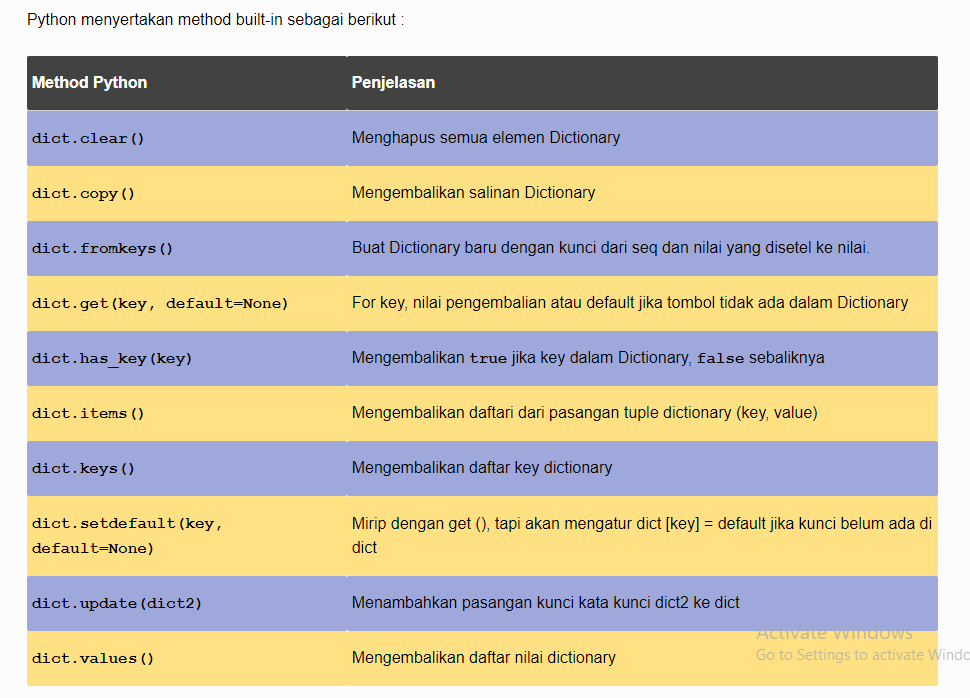
\includegraphics[width=0.70\textwidth]{figures/Method}}
	\caption{Method Build Dictionary Python}
	\label{Method Build Dictionary Python}
\end{figure}

\vspace{12pt}
Tipe data daftar memiliki beberapa metode lagi. Berikut adalah semua metode daftar objek: \par
\vspace{12pt}
\noindent 
list.append (x) \par
\noindent 
Tambahkan item ke bagian akhir daftar; setara dengan [len (a):] = [x]. \par
\vspace{12pt}
\noindent 
list.extend (L) \par
\noindent 
Perluas daftar dengan menambahkan semua item dalam daftar yang diberikan; setara dengan [len (a):] = L. \par
\vspace{12pt}
\noindent 
list.insert (i, x) \par
\noindent 
Masukkan item pada posisi tertentu. Argumen pertama adalah indeks dari elemen yang sebelum dimasukkan, jadi a.insert (0, x) memasukkan di bagian depan daftar, dan a.insert (len (a), x) setara dengan a.append ( x). \par
\vspace{12pt}
\noindent 
list.remove (x) \par
\noindent 
Hapus item pertama dari daftar yang nilainya x. Ini adalah kesalahan jika tidak ada item seperti itu. \par
\vspace{12pt}
\noindent 
list.pop ([i]) \par
\noindent 
Hapus item pada posisi yang diberikan dalam daftar, dan kembalikan. Jika tidak ada indeks yang ditentukan, a.pop () menghapus dan mengembalikan item terakhir dalam daftar. (Tanda kurung siku di sekitar i pada tanda tangan metode menunjukkan bahwa parameternya adalah opsional, bukankah Anda harus mengetikkan tanda kurung siku pada posisi itu. Anda akan sering melihat notasi ini di Referensi Perpustakaan Python.) \par
\vspace{12pt}
\noindent 
list.index (x) \par
\noindent 
Kembalikan indeks di daftar item pertama yang nilainya x. Ini adalah kesalahan jika tidak ada item seperti itu. \par
\vspace{12pt}
\noindent 
list.count (x) \par
\noindent 
Kembalikan berapa kali x muncul dalam daftar. \par
\vspace{12pt}
\noindent 
list.sort (cmp = None, key = None, reverse = False) \par
\noindent 
Urutkan item daftar di tempat (argumen dapat digunakan untuk kustomisasi sortir, lihat diurutkan () untuk penjelasan mereka). \par
\vspace{12pt}
\noindent 
list.reverse () \par
\noindent 
Membalik unsur daftar, di tempat. \par

\vspace{\baselineskip}
\vspace{\baselineskip}
\vspace{\baselineskip}
\vspace{\baselineskip}
\subsection{Dictionaries Introductions}
\vspace{\baselineskip}
\noindent Dictionaris\par


\noindent \hspace*{0.5in}Introductions\par


\noindent \hspace*{0.5in}Kami sudah mengenal daftar di bab sebelumnya. Di bab kursus Python online kami, kami \hspace*{0.5in}akan mempresentasikan kamus dan operator dan metode pada kamus. Program atau skrip \hspace*{0.5in}Python tanpa daftar dan kamus hampir tidak dapat dibayangkan. Seperti daftar kamus yang \hspace*{0.5in}bisa dengan mudah diubah, bisa menyusut dan berkembang ad libitum pada saat run time. \hspace*{0.5in}Mereka menyusut dan tumbuh tanpa perlu membuat salinan. Kamus dapat dimuat dalam \hspace*{0.5in}daftar dan sebaliknya. Tapi apa perbedaan antara daftar dan kamus? Daftar diurutkan dari \hspace*{0.5in}objek, sedangkan kamus tidak berurutan. Tapi perbedaan utamanya adalah item dalam \hspace*{0.5in}kamus diakses melalui kunci dan tidak melalui posisinya. Kamus adalah array asosiatif \hspace*{0.5in}(juga dikenal sebagai hash). Kunci kamus mana pun dikaitkan (atau dipetakan) ke sebuah \hspace*{0.5in}nilai. Nilai kamus bisa berupa tipe data Python. Jadi kamus adalah pasangan kunci-nilai \hspace*{0.5in}tak berurutan.\par


\vspace{\baselineskip}
\noindent \hspace*{0.5in}Kamus tidak mendukung urutan operasi dari jenis data urutan seperti string, tupel dan \hspace*{0.5in}daftar. Kamus termasuk tipe pemetaan built-in. Mereka adalah satu-satunya wakil \hspace*{0.5in}semacam ini!\par


\vspace{\baselineskip}
\noindent \hspace*{0.5in}Di akhir bab ini, kami akan menunjukkan bagaimana kamus dapat diubah menjadi satu \hspace*{0.5in}daftar, berisi (kunci, nilai) -tupel atau dua daftar, yaitu satu dengan kunci dan satu dengan \hspace*{0.5in}nilainya. Transformasi ini bisa dilakukan secara terbalik juga.\par

\vspace{\baselineskip}
\vspace{12pt}
\vspace{\baselineskip}

\noindent \hspace*{0.5in}Membuat kamus sama mudahnya dengan menempatkan item dalam kurung kurawal $ \{ $ $ \} $  \hspace*{0.5in}dipisahkan dengan koma. Item memiliki kunci dan nilai yang sesuai dinyatakan sebagai \hspace*{0.5in}pasangan, kunci: nilai. Sementara nilai dapat berupa tipe data apa pun dan dapat diulang, \hspace*{0.5in}kunci harus terdiri dari tipe yang tidak dapat diubah (string, number atau tupel dengan \hspace*{0.5in}elemen yang tidak berubah) dan harus unik.\par

\vspace{\baselineskip}
\vspace{12pt}
\noindent \hspace*{0.5in}Sementara pengindeksan digunakan dengan jenis wadah lain untuk mengakses nilai, kamus \hspace*{0.5in}menggunakan tombol. Kunci dapat digunakan baik di dalam tanda kurung siku atau dengan \hspace*{0.5in}metode get (). Perbedaan saat menggunakan get () adalah mengembalikan Elemen alih-alih \hspace*{0.5in}KeyError, jika kuncinya tidak ditemukan.\par

\vspace{\baselineskip}
\noindent \hspace*{0.5in}\hspace*{0.5in}my$ \_ $ dict = $ \{ $ 'name':'Jack', 'age': 26$ \} $ \par


\noindent \hspace*{0.5in}\hspace*{0.5in}$\#$  Output: Jack\par


\noindent \hspace*{0.5in}\hspace*{0.5in}print(my$ \_ $ dict['name'])\par


\noindent \hspace*{0.5in}\hspace*{0.5in}$\#$  Output: 26\par


\noindent \hspace*{0.5in}\hspace*{0.5in}print(my$ \_ $ dict.get('age'))\par


\noindent \hspace*{0.5in}\hspace*{0.5in}$\#$  Trying to access keys which doesn't exist throws error\par


\noindent \hspace*{0.5in}\hspace*{0.5in}$\#$  my$ \_ $ dict.get('address')\par


\noindent \hspace*{0.5in}\hspace*{0.5in}$\#$  my$ \_ $ dict['address']\par


\noindent \hspace*{0.5in}Saat menjalankan program, hasilnya adalah:\par


\noindent \hspace*{0.5in}\hspace*{0.5in}Jack\par


\noindent \hspace*{0.5in}\hspace*{0.5in}26\par


\vspace{\baselineskip}

\vspace{\baselineskip}
\vspace{\baselineskip}



